%% Conversational MURENA -- EDBT 2027 demo paper, editable LaTeX source.
%% Evaluation section describes the v3 three-condition protocol
%% (refined / one_shot / oracle). Measured v3 results are NOT inserted:
%% search for "RESULTS-PENDING" to find the blocks to fill.
\documentclass[sigconf,review]{acmart}
\geometry{twoside=true, head=13pt, a4paper, includeheadfoot,
 columnsep=2pc, top=57pt, bottom=73pt, inner=54pt, outer=54pt,
 marginparwidth=2pc, heightrounded}
\AtBeginMaketitle{%% EDBT Conference Proceedings setup for ACM sigconf Style



%% EDBT: ISBN and year have to be adapted with every Number / Volume !
%%
\def\EDBTISSN{xxxx-xxxx}
\def\EDBTISBN{xxx-x-xxxxx-xxx-x}
\setcopyright{none}
\copyrightyear{\copyright\ 2027 Copyright held by the owner/author(s).
  Published on xxxxx under ISBN \EDBTISBN, series ISSN \EDBTISSN.
  Distribution of this paper is permitted under the terms of the
  Creative Commons license CC-by-nc-nd 4.0}
\acmYear{2027}
\acmDOI{}
\acmISBN{}


%% These commands are for a PROCEEDINGS abstract or paper.
%% EDBT: This needs adaptation every year!
\acmConference[EDBT '27]{Extending Database Technology}{6-9 April 2027}{Lille (France)}
%%
%%  Uncomment \acmBooktitle if the title of the proceedings is different
%%  from ``Proceedings of ...''!
%%
%%\acmBooktitle{Woodstock '18: ACM Symposium on Neural Gaze Detection,
%%  June 03--05, 2018, Woodstock, NY}


%% EDBT:
\settopmatter{printacmref=false, printccs=false, printfolios=false}


%% EDBT:
%% Macro to make image usable as hyperlink [see http://tex.stackexchange.com/questions/31819/xelatex-includegraphics-and-hyperlink]
\newsavebox{\ximagebox}
\newlength{\ximageheight}
\newsavebox{\xglyphbox}
\newlength{\xglyphheight}
\newcommand{\xbox}[1]%
  {\savebox{\ximagebox}{#1}%
  \settoheight{\ximageheight}{\usebox{\ximagebox}}%
  \savebox{\xglyphbox}{\color{white}\char32}%
  \settoheight{\xglyphheight}{\usebox{\xglyphbox}}%
  \raisebox{\ximageheight}[0pt][0pt]{\raisebox{-\xglyphheight}[0pt][0pt]{%
    \makebox[0pt][l]{\usebox{\xglyphbox}}}}%
    \usebox{\ximagebox}%
    \raisebox{0pt}[0pt][0pt]{\makebox[0pt][r]{\usebox{\xglyphbox}}}}

%% now use this to define the logo header:

\newsavebox{\LogoBox}
\sbox{\LogoBox}{}

%% now define our header and footer for the first page
\fancypagestyle{firstpagestyle}{%
  \fancyhf{}%
  \fancyfoot{}%
  \fancyhead[L,C]{}
  \fancyhead[R]{}{\raisebox{15pt}[0pt][0pt]{\xbox{\usebox{\LogoBox}}}}
  }

\hypersetup{%
  pdfcopyright={CC-by-nc-nd},
  pdfcreator={LaTeX with acmart, hyperref, and EDBT modifications},
  pdfvolumenum={XX},
  pdfissuenum={X},
  pdfisbn={\EDBTISBN},
  pdfissn={\EDBTISSN}
}
}
\usepackage{tikz}
\usetikzlibrary{arrows.meta,positioning,fit,backgrounds}
\usepackage{pgfplots}
\pgfplotsset{compat=1.18}
%% Placeholder for pending v3 numbers (used only inside RESULTS-PENDING).
\newcommand{\RP}{\textbf{??}}
%% Keep only rows whose column #1 equals #2 (used by the per-k figure).
\pgfplotsset{discard if not/.style 2 args={x filter/.append code={%
  \edef\tempa{\thisrow{#1}}\edef\tempb{#2}%
  \ifx\tempa\tempb\else\def\pgfmathresult{inf}\fi}}}
\setlength{\emergencystretch}{1.5em}
\begin{document}
\title{Conversational MURENA: Clarifying Underspecified Requests for Real-Estate Portfolio Screening}
\author{Authors to be confirmed}
\affiliation{\institution{Affiliations to be confirmed}\city{Turin}\country{Italy}}
\renewcommand{\shortauthors}{Authors to be confirmed}

\begin{abstract}
MURENA translates natural-language requests into structured requirements,
database searches, and explainable real-estate portfolio rankings, but
assumes that the initial request is sufficiently specified. We demonstrate
a conversational stage that clarifies unresolved requirements
\emph{before} the original multi-agent pipeline runs. It tracks the state
of MURENA's six query dimensions, separates unconfirmed omissions from
explicit non-preferences, asks one targeted question per turn in an order
inspired by the EVPI criterion of SAGE-Agent, and requires the user to
review and confirm a rewritten request. Query template, agents, SQL
construction, and ranking are inherited unchanged. We describe a
controlled-omission benchmark (8 intents, 0--5 omitted dimensions, 48
scenarios) that compares refined, one-shot, and complete (oracle) queries
under the same pipeline, and report robustness observations from an
earlier 24-scenario suite. Two demonstration paths let attendees see how
clarification changes the interpreted request and the resulting
portfolio screening.
\end{abstract}
\keywords{conversational query clarification, requirement elicitation,
real-estate decision support, multi-agent systems, text-to-SQL}
\maketitle

\section{Introduction}
\label{sec:intro}
MURENA~\cite{deluca2026murena} supports large-scale real-estate screening
through natural-language input, specialized domain agents, SQL-based
filtering, multi-criteria scoring, and explanations. Its paper
acknowledges that the approach assumes a sufficiently specified initial
request. Real tasks often start from a broad objective: a user may state
a future use for a building without the floor area, energy, or location
criteria that matter to the decision, and the pipeline then silently
runs without them.

Omission is not always an error. MURENA's dimensions are optional, and a
user may genuinely have no preference about energy class. The problem is
therefore not to fill every field, but to tell which information is
still unresolved and to obtain a request the user has confirmed.

We present \emph{Conversational MURENA}, a pre-analysis clarification
stage that neither adds query dimensions nor changes retrieval and
ranking. The demonstration contributes (i)~stateful elicitation over the
existing dimensions with explicit recording of non-preferences,
(ii)~a question order adapted from the SAGE-Agent
method~\cite{suri2026sage} and a mandatory review step, (iii)~a three-condition benchmark protocol that
separates the cost of missing information from the effectiveness and
cost of recovering it, and (iv)~guided and open-ended demonstration
paths.

\section{Related Work}
\label{sec:related}
\emph{Clarification in LLMs.} CLAMBER~\cite{zhang2024clamber} shows
that LLMs are weak at \emph{identifying} ambiguous information needs,
and QuestBench~\cite{li2025questbench} casts clarification as finding
the minimal necessary question in underspecified reasoning tasks.
SAGE-Agent~\cite{suri2026sage} models uncertainty over tool parameters,
ranks candidate questions by expected value of perfect information
(EVPI), and penalizes redundant questions on the same aspect; our
question ordering adapts this idea heuristically.
\emph{Ambiguity and interaction for data access.}
AmbiQT~\cite{bhaskar2023ambiqt}, AMBROSIA~\cite{saparina2024ambrosia},
and PRACTIQ~\cite{dong2025practiq} benchmark ambiguous or unanswerable
text-to-SQL questions; AMBROSIA also reports that LLMs struggle to
recognize ambiguity. AmbiSQL~\cite{ding2026ambisql} demonstrates
multiple-choice clarification before SQL generation,
FISQL~\cite{menon2025fisql} refines SQL through user feedback, and
COOL~\cite{francia2021cool} disambiguates conversational OLAP sessions.
These systems resolve ambiguity with respect to a database schema or a
generated query. We instead elicit \emph{domain requirements} for a
fixed six-dimension template (use, location, building, energy,
proximity) before a multi-agent screening pipeline, and evaluate
recovery per dimension and through its effect on the ranked portfolio.

\section{System}
\label{sec:system}
\paragraph{Inherited pipeline.} MURENA represents a request as
$Q=(I,D,L,\allowbreak C_b,C_e,C_p)$: property type or search intent $I$, intended
use $D$, location $L$, building and capacity constraints $C_b$, energy
requirements $C_e$, and service proximity $C_p$. Specialized agents
extract each dimension, an SQL agent builds relational and spatial
filters, and candidates are scored and ranked with explanations shown on
a map (Fig.~\ref{fig:arch}, bottom). This part is unchanged.

\begin{figure}[t]
\centering
\resizebox{\columnwidth}{!}{%% Architecture of Conversational MURENA (TikZ, one column).
%% New components: solid border, grey fill. Inherited MURENA components:
%% solid border, white fill. The state row shows the MS02_k2 example
%% (nursery request with C_b and C_e omitted).
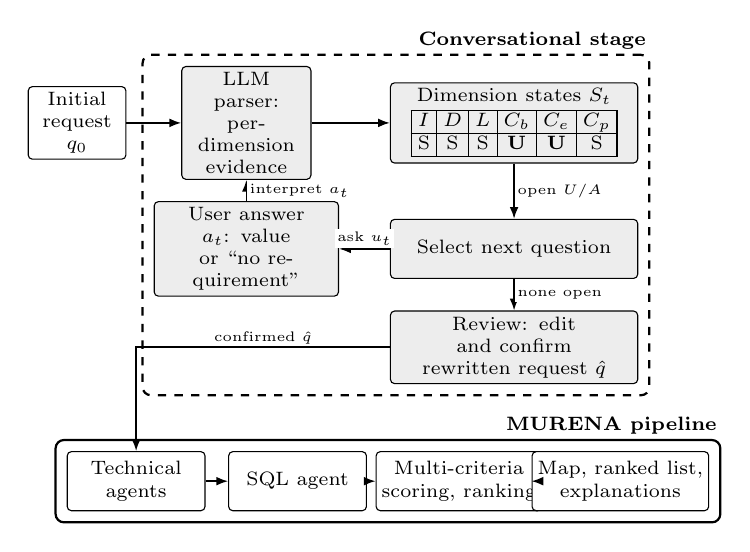
\begin{tikzpicture}[
  font=\scriptsize,
  box/.style={draw, rounded corners=1.5pt, align=center, inner sep=2pt,
    minimum height=7.5mm},
  new/.style={box, fill=black!7},
  old/.style={box, fill=white, minimum width=17.5mm},
  arr/.style={-{Latex[length=1.5mm]}, semithick},
  lbl/.style={font=\tiny, inner sep=1pt, fill=white},
]
% --- conversational stage (new) ---
\node[box, text width=11mm] (q0) at (0,0) {Initial\\request $q_0$};
\node[new, text width=15mm] (parse) at (2.15,0)
  {LLM parser:\\per-dimension\\evidence};
\node[new, text width=30mm] (state) at (5.55,0)
  {Dimension states $S_t$\\[1pt]
   \setlength{\tabcolsep}{2.2pt}%
   \begin{tabular}{|c|c|c|c|c|c|}\hline
   $I$ & $D$ & $L$ & $C_b$ & $C_e$ & $C_p$\\\hline
   S & S & S & \textbf{U} & \textbf{U} & S\\\hline
   \end{tabular}};
\node[new, text width=30mm] (select) at (5.55,-1.6)
  {Select next question};
\node[new, text width=22mm] (answer) at (2.15,-1.6)
  {User answer $a_t$: value\\or ``no requirement''};
\node[new, text width=30mm] (review) at (5.55,-2.85)
  {Review: edit and confirm\\rewritten request $\hat q$};

\draw[arr] (q0) -- (parse);
\draw[arr] (parse) -- (state);
\draw[arr] (state) -- node[lbl, right] {open $U$/$A$} (select);
\draw[arr] (select) -- node[lbl, above] {ask $u_t$} (answer);
\draw[arr] (answer) -- node[lbl, right] {interpret $a_t$} (parse);
\draw[arr] (select) -- node[lbl, right] {none open} (review);

% --- inherited MURENA pipeline ---
\node[old] (agents) at (0.75,-4.55) {Technical\\agents};
\node[old] (sql) at (2.8,-4.55) {SQL agent};
\node[old] (rank) at (4.85,-4.55) {Multi-criteria\\scoring, ranking};
\node[old] (map) at (6.9,-4.55) {Map, ranked list,\\explanations};
\draw[arr] (agents) -- (sql);
\draw[arr] (sql) -- (rank);
\draw[arr] (rank) -- (map);
\draw[arr] (review.west) -| node[lbl, pos=0.25, above] {confirmed $\hat q$}
  (agents.north);

\begin{scope}[on background layer]
  \node[draw, dashed, thick, rounded corners=3pt, inner sep=4pt,
    fit=(parse)(state)(select)(answer)(review),
    label={[font=\scriptsize\bfseries, anchor=south east, inner sep=1.5pt]
      north east:Conversational stage}] (gnew) {};
  \node[draw, thick, rounded corners=3pt, inner sep=4pt,
    fit=(agents)(sql)(rank)(map),
    label={[font=\scriptsize\bfseries, anchor=south east, inner sep=1.5pt]
      north east:MURENA pipeline}] (gold) {};
\end{scope}
\end{tikzpicture}
}
\caption{Conversational stage (dashed, grey) feeding the inherited MURENA
pipeline (solid). The state row shows the guided demo request: intent,
use, location, and proximity specified (S); $C_b$ and $C_e$ unconfirmed
absent (U); A marks ambiguous. Only the confirmed text $\hat q$ reaches the pipeline.}
\Description{Block diagram. An initial request enters an LLM parser,
which produces six dimension states. While a state is unconfirmed or
ambiguous, a question is selected and asked, and the user's answer is
interpreted and updates the states. When none is open, the user reviews
and confirms a rewritten request, which is passed to the inherited
pipeline of six dimension agents, SQL and spatial filters, scoring and
ranking, and a map with explanations. New components have dashed
borders and grey fill; inherited ones have solid borders.}
\label{fig:arch}
\end{figure}

\paragraph{Dimension states.} An LLM parser assigns each dimension one
of five states: \emph{specified}, \emph{ambiguous},
\emph{unconfirmed absent}, \emph{not requested}, or \emph{missing
critical}. A plain omission becomes \emph{unconfirmed absent}; only an
explicit user statement makes it \emph{not requested}, so an omission is
never silently read as a non-preference. Dimension boundaries follow
MURENA: $C_b$ is specified only by requirements that filter properties
(floor area, capacity, explicit structural features); words that merely
name the property or its status, such as ``existing building'', do not
specify $C_b$. A stated capacity remains part of $C_b$ and is not
converted into a floor-area filter.

\paragraph{Question selection.} Every unconfirmed omission or blocking
ambiguity yields a candidate question, whose wording the LLM generates;
for $D$ it may suggest up to two intended uses from the regulatory
catalogue, and for $L$ up to three candidate cities, marked as unverified
and always with an ``other city'' option. One question is asked per
turn. Following SAGE-Agent~\cite{suri2026sage}, candidates with
enumerable alternatives are ordered by an EVPI-style score over uniform
weights, minus a penalty for each earlier question on the same aspect.
This is an \emph{ordering heuristic}: weights are not calibrated
posteriors, nothing is trained, and the score does not decide
readiness: every unconfirmed omission must be answered or explicitly
declined before analysis. A turn limit (six by default) blocks sessions that
cannot be resolved.

\paragraph{Answers and review.} The LLM classifies each answer
(requirement, opt-out, unknown, rejection of the offered options, or
unclear) and extracts per-dimension updates with an evidence span; state
updates are then deterministic. Unclear answers trigger a rephrased
follow-up, and a separate check blocks answers that contradict earlier
requirements. Transient model failures are reported as retryable errors
that keep the session alive. When no dimension is open, the LLM rewrites
the request into $\hat q$ from the original text and confirmed answers;
the user edits and confirms it, and only this text is passed to the
pipeline. LLM interpretation can still err; the review step is the
user's safeguard, not a guarantee.

\paragraph{Regulatory catalogue.} A source-documented catalogue of eight
intended uses (five early-childhood services, two care services for
older adults, and a student residence tied to a specific public funding
programme) supplies use examples and lets the regulatory agent match
uses. It is supporting coverage, not a new query template: matching a
use is distinct from deciding whether a provision applies, neither is a
compliance certification, and user-defined gross floor area is not
confused with room-level legal measures.

\section{Demonstration}
\label{sec:demo}
Attendees use the web interface: a conversation panel shows each
generated question, possibly with suggested options, and accepts a
free-text answer, including ``no requirement''; a review form shows the
editable rewritten request with a \emph{Confirm and start analysis}
button; the result view shows candidates on a map with a ranked,
explained list. The per-dimension state of Fig.~\ref{fig:arch} is
maintained by the backend; the presenter uses the figure to explain
which questions are asked and why.
\begin{figure*}[t]\centering
\begin{minipage}[b]{0.43\textwidth}\centering
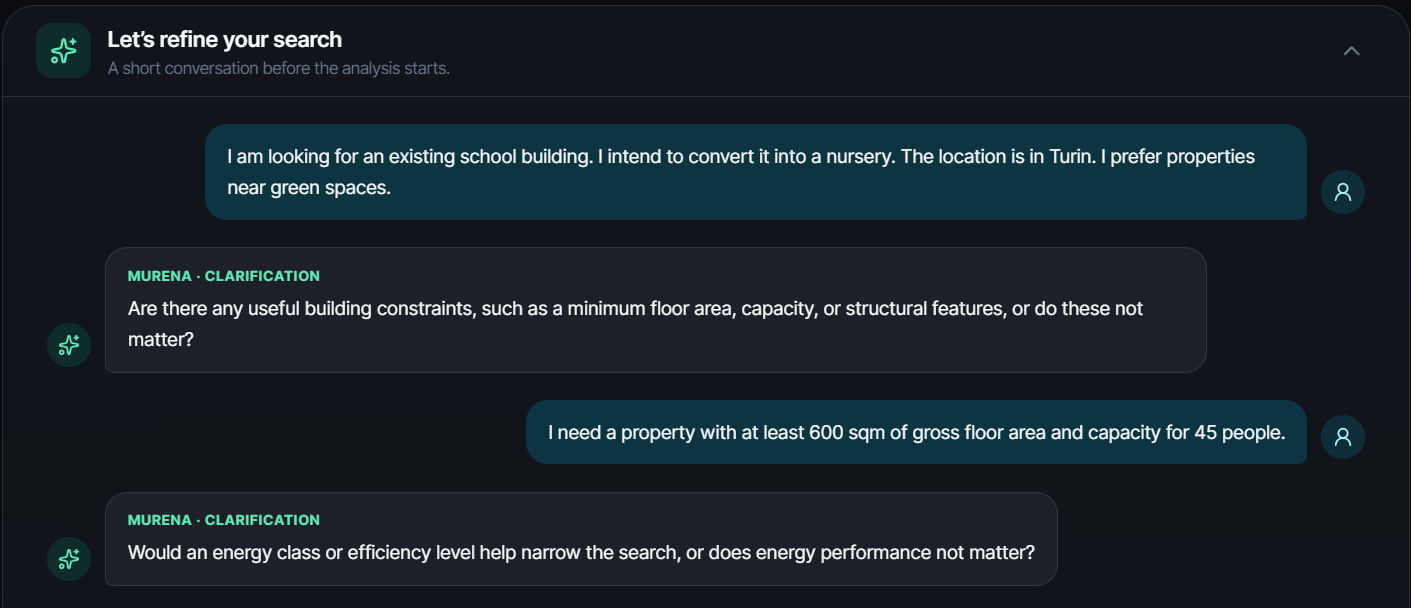
\includegraphics[width=\linewidth]{figures/screen-dialogue.png}\\[2pt]
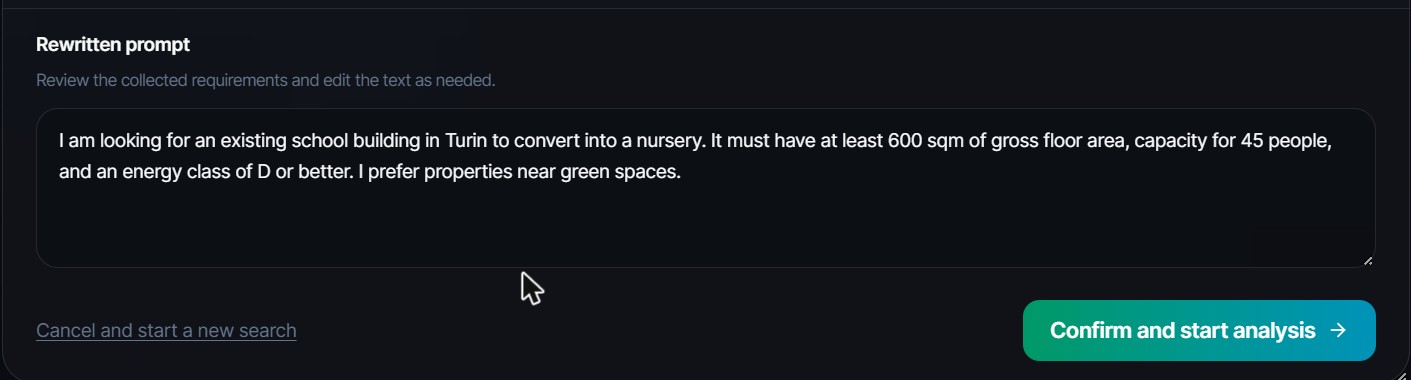
\includegraphics[width=\linewidth]{figures/screen-review.png}\\
{\footnotesize (a) Clarification dialogue and review form}
\end{minipage}\hfill
\begin{minipage}[b]{0.55\textwidth}\centering
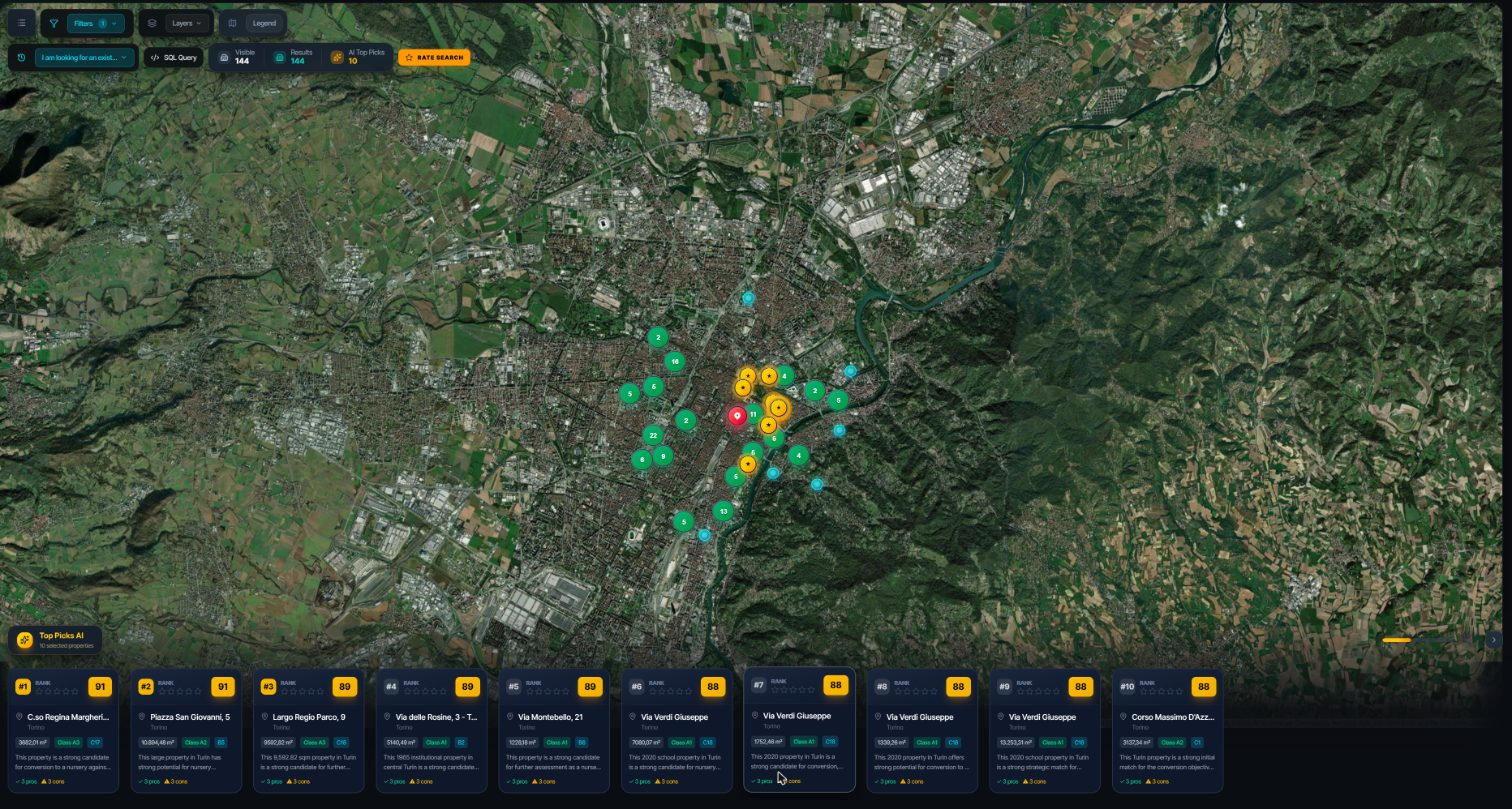
\includegraphics[width=\linewidth]{figures/screen-results.jpg}\\
{\footnotesize (b) Map and ranked candidates after confirmation}
\end{minipage}
\caption{Guided path captured on the running system:
the system asks only for the two unconfirmed dimensions
($C_b$, $C_e$), the attendee confirms the rewritten request, and the
inherited pipeline returns 144 matching properties with a ranked top-10.}
\Description{Left: chat panel with the nursery request, a question on
building constraints, the answer with floor area and capacity, a question
on energy class, and the editable rewritten prompt with a confirm button.
Right: satellite map of Turin with clustered result markers and a strip
of ten ranked property cards.}
\label{fig:screens}
\end{figure*}

\paragraph{Guided path: nursery conversion.} The attendee submits ``an
existing school building in Turin to convert into a nursery, near green
spaces''. Intent, use, location, and proximity are specified, while
floor area and capacity ($C_b$) and energy class ($C_e$) are
unconfirmed; ``existing building'' does not count as a $C_b$
requirement. The system asks two questions, one per dimension; the
attendee states a minimum floor area and capacity, and either an energy
class or that energy does not matter. The review form shows the
rewritten request, which the attendee edits or confirms; the inherited
pipeline then exposes the extracted filters, the candidates on the map,
and the ranked explanations (Fig.~\ref{fig:screens}). This path
corresponds to a benchmark scenario ($k=2$) whose two-turn dialogue was
observed in a functional check and in the live session of
Fig.~\ref{fig:screens}.

\paragraph{Open-ended path: student residence.} Visitors start from a
broad renovation objective, specify student housing, and decide whether
the specific public funding programme in the catalogue is relevant. The
dialogue separates user-stated building preferences from programme
conditions, and different answers yield different confirmed requests
and portfolios. Open-ended interaction is not claimed to be reproducible
across arbitrary attendee choices.

\section{Evaluation}
\label{sec:eval}
\paragraph{Scenarios.} The controlled-omission benchmark (v3) starts
from eight fully specified reference intents $q^*$, one per catalogue
use. For each intent, nested initial queries $q_0$ omit
$k\in\{1,\dots,5\}$ of the dimensions $D,L,C_b,C_e,C_p$ ($I$ is always
kept), in an omission order that differs across intents; $k=0$ controls
contain all six. This gives 48 scenarios, eight per level. In v3 the
capacity is stated inside the $C_b$ fragment with a use-neutral noun, so
omitting $C_b$ removes it from $q_0$; in the earlier v2 family it leaked
through the use phrase. The simulated user answers each question with
the omitted fragment for the targeted dimension.

\paragraph{Conditions.} \emph{Refined}: $q_0$ goes through
clarification with the simulated user, the rewritten $\hat q$ is
accepted without edits, and $\hat q$ (never $q^*$) is analysed; all 48
scenarios, 3 repetitions. \emph{One-shot}: $q_0$ is analysed directly;
40 scenarios with $k\ge1$, 3 repetitions. \emph{Oracle}: $q^*$ is
analysed directly, 5 repetitions per intent. This yields 304 runs in a
seeded interleaved order, all with the same code version, pipeline
options (including MURENA's result relaxation, whose activation is
logged), and the 89,200-property MURENA dataset. Run-to-run variability
is measured rather than assumed absent. The oracle ranking is a
\emph{reference query output}, not ground truth on property relevance.

\paragraph{Metrics.} \emph{Clarification}: precision, recall, and $F_1$
of detecting the initially omitted dimensions; number of turns;
completion; the rate of unnecessary turns at $k=0$. \emph{Ranking
agreement with the oracle}: Jaccard similarity of the top-5 sets ($J_5$)
and extrapolated rank-biased overlap~\cite{webber2010rbo} ($p=0.8$) over
the stored top-10, averaged over all condition-by-oracle repetition
pairs. The same metrics between oracle repetitions give a \emph{noise
ceiling}. Because scores are coarse, a tie-aware variant averages over
1,000 random permutations within equal-score groups. Pairs with two
empty results are excluded and reported; one empty side scores 0.
\emph{Structured filter agreement}: per-dimension atoms extracted by the
agents before relaxation (e.g., use, city and radius, minimum area,
worst admitted energy class, proximity category) are compared with the
atoms present in a strict majority of oracle repetitions ($F_1$,
per-dimension recall, invented atoms). \emph{Cost}: latency split into
clarification and analysis. Per-level means carry 95\% percentile
intervals from a cluster bootstrap over the eight intents
($B=10{,}000$); the intent-level difference refined~$-$~one-shot is
tested with an exact sign-flip test.

\paragraph{Scope.} The simulated user reveals exactly what was omitted,
so refined-versus-oracle agreement is an upper bound on recovery rather
than evidence about real users; the comparison measures the value of
the added information, not of dialogue over a static form. The level
$k$ is coupled to the identity of the omitted dimensions, so results
are stratified by $k$ and not read as a causal effect of the count. At
$k=0$, $q_0$ and $q^*$ differ only in wording, which bounds
wording-induced variation.

%% ===================== RESULTS-PENDING (v3) =====================
%% Fill from backend/experiments/results/missingness_v3 (compare_conditions.py
%% and the per-k CSV). Remove \iffalse/\fi once numbers are verified and
%% documented in docs/okf/research/edbt-conversational-benchmark.md.
%% Labels: tab:results, fig:perk. Data file: data/per_k.csv with columns
%% k,cond,j5,j5_lo,j5_hi,rbo,rbo_lo,rbo_hi (cond in {one_shot,refined,
%% oracle}; oracle rows hold the oracle-vs-oracle noise ceiling).
\iffalse
\paragraph{Results.} Table~\ref{tab:results} and Fig.~\ref{fig:perk}
summarize the 304 runs. % RESULTS-PENDING: 3-5 sentences, no claims
% beyond the measured values and CIs; report completion and errors.

\begin{table}[t]
\caption{v3 benchmark ($k\ge1$ unless noted): mean [95\% cluster-bootstrap CI].}
\label{tab:results}
\centering\scriptsize\setlength{\tabcolsep}{3pt}
\begin{tabular}{@{}lccccc@{}}
\toprule
Condition & $J_5$ & RBO & Filter $F_1$ & Turns & Latency (s) clar./anal.\\
\midrule
One-shot & \RP & \RP & \RP & -- & -- / \RP\\
Refined & \RP & \RP & \RP & \RP & \RP / \RP\\
Refined, $k=0$ & \RP & \RP & \RP & \RP & \RP / \RP\\
Oracle vs.\ oracle & \RP & \RP & \RP & -- & -- / \RP\\
\midrule
$\Delta$ refined$-$one-shot & \RP & \RP & \RP & & \\
Sign-flip $p$ & \RP & \RP & \RP & & \\
\bottomrule
\end{tabular}
\\[2pt]
Detection P/R/$F_1$: \RP; unnecessary-turn rate at $k=0$: \RP;
tie-aware $J_5$: \RP; completion: \RP.
\end{table}

\begin{figure}[t]
\centering
\begin{tikzpicture}
\begin{axis}[width=\columnwidth, height=40mm, xlabel={omitted dimensions $k$},
  ylabel={$J_5$ vs.\ oracle}, xmin=-0.3, xmax=5.3, ymin=0, ymax=1,
  xtick={0,...,5}, legend pos=south west, legend style={font=\scriptsize},
  tick label style={font=\scriptsize}, label style={font=\scriptsize}]
\addplot+[mark=square*, error bars/.cd, y dir=both, y explicit]
  table[x=k, y=j5, col sep=comma, discard if not={cond}{refined},
  y error plus expr=\thisrow{j5_hi}-\thisrow{j5},
  y error minus expr=\thisrow{j5}-\thisrow{j5_lo}] {data/per_k.csv};
\addlegendentry{refined}
\addplot+[mark=triangle*, error bars/.cd, y dir=both, y explicit]
  table[x=k, y=j5, col sep=comma, discard if not={cond}{one_shot},
  y error plus expr=\thisrow{j5_hi}-\thisrow{j5},
  y error minus expr=\thisrow{j5}-\thisrow{j5_lo}] {data/per_k.csv};
\addlegendentry{one-shot}
\addplot+[dashed, mark=none, black]
  table[x=k, y=j5, col sep=comma, discard if not={cond}{oracle}]
  {data/per_k.csv};
\addlegendentry{oracle vs.\ oracle}
\end{axis}
\end{tikzpicture}
\caption{Top-5 agreement with the oracle per omission level (mean and
95\% cluster-bootstrap CI over 8 intents). An RBO panel uses the
\texttt{rbo}, \texttt{rbo\_lo}, \texttt{rbo\_hi} columns.}
\Description{Line chart of top-5 Jaccard agreement with the oracle
against the number of omitted dimensions, for refined and one-shot
queries, with the oracle-vs-oracle noise ceiling as a dashed line.}
\label{fig:perk}
\end{figure}
\fi
%% =================== END RESULTS-PENDING (v3) ===================

\paragraph{Earlier robustness suite.} A separate suite of 24 synthetic
scenarios covers single omissions, ambiguous uses and locations,
explicit non-preferences, an out-of-catalogue use, and funding-scope
cases. It was run on 2026-11-16 in the conversational condition only
(3 repetitions, 72 runs, an earlier code version
preceding the current pipeline fixes). All runs completed; detection of
initially missing dimensions reached micro precision 1.00, recall 0.90,
and $F_1$ 0.95 (64/72 exact). The failures are instructive. Two
ambiguous-use requests (an ``elder-care facility'' and a ``service for
young children'') were never flagged as ambiguous (0/6 exact): the
system asked only about the omitted dimension. This is consistent with
the detection difficulty reported by CLAMBER and
AMBROSIA~\cite{zhang2024clamber,saparina2024ambrosia}. For a
co-housing request outside the catalogue, the regulatory agent wrongly
matched the student-residence use in all 3 runs. These runs measure
neither the benefit of clarification nor ranking quality.

\section{Conclusion}
\label{sec:conclusion}
Conversational MURENA addresses the original assumption of a
sufficiently specified request without changing the query template or
the ranking method: unresolved dimensions are made explicit, answered or
declined, and confirmed by the user before analysis. The demonstration
shows this interaction live, and the three-condition benchmark separates
the cost of missing information from its recovery. Limitations remain:
ambiguity detection is weaker than omission detection, the simulated
user is cooperative and exact, no static-form baseline isolates the
contribution of dialogue, and agreement with an oracle query is not
independently judged relevance. A user study and a form-based baseline
are natural next steps.

\bibliographystyle{ACM-Reference-Format}
\bibliography{sample-base}
\end{document}
